\documentclass[12pt]{article}

%IMPORTS
\usepackage[catalan]{babel}
\usepackage[utf8]{inputenc}
\usepackage{graphicx}
\usepackage{wrapfig}
\usepackage{amsmath}
\usepackage{amssymb}
\usepackage{ragged2e} 
\usepackage{subfig}
\usepackage{caption}
\usepackage{subcaption}
%\usepackage[usenames]{color}
\usepackage[dvipsnames]{xcolor}
\usepackage{float}
\usepackage{chngcntr}
\usepackage{ragged2e}
\usepackage{multirow}
\usepackage{vmargin}
\usepackage{hyperref}
\usepackage{url}
\usepackage{fancyhdr}
\usepackage{bigints}

\definecolor{navy}{rgb}{0,0,128}

\setpapersize{A4}
\setmargins{2.5cm}     % margen izquierdo
{2.6cm}                % margen superior
{16.5cm}               % anchura del texto
{23.7cm}               % altura del texto
{10pt}                 % altura de los encabezados
{0cm}                  % espacio entre el texto y los encabezados
{0pt}                  % altura del pie de página
{1cm}                  % espacio entre el texto y el pie de página
\renewcommand{\baselinestretch}{1.5}

\begin{document}

\begin{titlepage}
    \centering
    {\bfseries\LARGE Universitat Autònoma de Barcelona\newline Facultat de Ciències\par}
    \vspace{2cm}
    {\hspace{-1em}
\includegraphics[width=0.4\textwidth]{logo.png}\par}
    \vspace{1cm}
    {\scshape\Huge Pràctica 1\par} %Fiat ut Nix --- et non erit nix
    \vspace{1cm}
    {\Large \itshape Autors: \par}
    {\Large \hspace{-1.75em} Gerard Lahuerta \& Ona Sánchez \par}
    {\Large 1601350 --- 1601181 \par}
    \vspace{1cm}
    {\Large 28 de Març del 2022\par}
\end{titlepage}

\justifying

\newpage
\setcounter{page}{2}
\pagestyle{plain}
\tableofcontents
\cleardoublepage
\addcontentsline{}{chapter}{}
\newpage
\section{Presentació de la llibreria i informació d'interés}\label{pres.llib}
La llibreria de funcions ha estat programada en llenguatge $C$ i consta de dos fitxers, un fitxer capcelera i un amb el codi de les funcions.\\
Per al seu funcionament precisa de les llibreries de $C$ \textcolor{LimeGreen}{math.h} i \textcolor{LimeGreen}{limits.h}.\\
També, el fitxer capcelera té definides les constants:
\begin{itemize}
    \item \textcolor{Dandelion}{E\_NUM\_SUBINTER}: missatge d'error per nombre d'intervals introduït com a \\paràmetre inferior a 1.
    \item \textcolor{Dandelion}{E\_FUNC}: missatge d'error per apuntador de funció introduïda per paràmetre $NULL$.
    \item \textcolor{Dandelion}{E\_NUM\_SUBINTER\_LEG}: missatge d'error per coeficients del nombre d'intervals \\introduït com a paràmetre no disponible en memòria.
\end{itemize}
La llibreria té programades quatre funcions que permeten calcular numèricament integrals de variable real. Totes retornen el valor de la integral o, en cas d'error, el valor $LLONG\_MAX$; ambdos casos serà de tipus \textbf{\textcolor{Turquoise}{double}} el valor retornat. \\
Recalcar a més, que cada funció conté el seu $CDocs$ propi que conté la informació més rellevant de la funció de manera resumida: \textit{input, output, descripció i informació rellevant}.
\newpage
\section{Presentació de les funcions}\label{ap2}
La llibreria creada en aquesta pràctica consta de 4 funcions, cada una amb un mètode d'integració numèrica. El mètodes implementats son els següents:
\subsection{Trapezi (Compost)}
\begin{itemize}
    \item Entrada:
    \begin{itemize}
        \item[$\circ$] Funció a integrar: \textbf{\textcolor{Turquoise}{double}} *f (\textbf{\textcolor{Turquoise}{double}},  *\textbf{\textcolor{Turquoise}{void}}).
        \item[$\circ$] Paràmetres que es passaran a la funció: \textbf{\textcolor{Turquoise}{void}} *params.
        \item[$\circ$] Valor inferior de la integral: \textbf{\textcolor{Turquoise}{double}} x0.
        \item[$\circ$] Valor superior de la integral: \textbf{\textcolor{Turquoise}{double}} xn.
        \item[$\circ$] Nombre de subintervals: \textbf{\textcolor{Turquoise}{int}} n.
    \end{itemize}
    \item Sortida:
        \begin{itemize}
            \item[$\circ$] Valor de la integral pel mètode del Trapezi: \textbf{\textcolor{Turquoise}{double}} area.
        \end{itemize}
    \item Funcionament:
    Un cop cridada la funció amb els paràmetres corresponents, es calcula el valor de la integral segons la següent expressió (mètode d'integració del Trapezi compost):
    \begin{equation*}
        \int_{x_0}^{x_n}f(x)dx \approx \frac{x_n-x_0}{2n}\left(f(x) + 2\sum_{i=1}^{n-1}f(x_i) + f(x_n)\right)
    \end{equation*}
    
    En el programa, la funció $f$ ve introduïda com a paràmetre en forma d'atribut pel que qualsevol programa que incorpori la llibreria pot enviar-li la fòrmula a integrar a la funció.
    
\end{itemize}
\newpage
\subsection{Simpson (Compost)}
\begin{itemize}
    \item Entrada:
    \begin{itemize}
        \item[$\circ$] Funció a integrar: \textbf{\textcolor{Turquoise}{double}} *f (\textbf{\textcolor{Turquoise}{double}},  *\textbf{\textcolor{Turquoise}{void}}).
        \item[$\circ$] Paràmetres que es passaran a la funció: \textbf{\textcolor{Turquoise}{void}} *params.
        \item[$\circ$] Valor inferior de la integral: \textbf{\textcolor{Turquoise}{double}} x0.
        \item[$\circ$] Valor superior de la integral: \textbf{\textcolor{Turquoise}{double}} x2n.
        \item[$\circ$] Nombre de subintervals: \textbf{\textcolor{Turquoise}{int}} n.
    \end{itemize}
    \item Sortida:
        \begin{itemize}
            \item[$\circ$] Valor de la integral pel mètode del Simpson: \textbf{\textcolor{Turquoise}{double}} area.
        \end{itemize}
    \item Funcionament:
    Un cop cridada la funció amb els paràmetres corresponents, es calcula el valor de la integral segons la següent expressió (mètode d'integració de Simpson compost):
       \begin{equation*}
            \int_{x_0}^{x_{2n}}f(x)dx \approx \frac{x_{2n}-x_0}{3\cdot 2n} \left(f(x_0) + f(x_2_n) + 4\sum_{i=0}^{n-1}f(x_{2i+1}) + 2\sum_{i=1}^{n-1}f(x_{2i})\right)
        \end{equation*}
        En el programa, la funció $f$ ve introduïda com a paràmetre en forma d'atribut pel que qualsevol programa que incorpori la llibreria pot enviar-li la fòrmula a integrar a la funció.

    
\end{itemize}
\newpage
\subsection{Legendre}
\begin{itemize}
    \item Entrada:
    \begin{itemize}
        \item[$\circ$] Funció a integrar: \textbf{\textcolor{Turquoise}{double}} *f (\textbf{\textcolor{Turquoise}{double}},  *\textbf{\textcolor{Turquoise}{void}}).
        \item[$\circ$] Paràmetres que es passaran a la funció: \textbf{\textcolor{Turquoise}{void}} *params.
        \item[$\circ$] Valor inferior de la integral: \textbf{\textcolor{Turquoise}{double}} x0.
        \item[$\circ$] Valor superior de la integral: \textbf{\textcolor{Turquoise}{double}} xn.
        \item[$\circ$] Nombre de subintervals: \textbf{\textcolor{Turquoise}{int}} n.
    \end{itemize}
    \item Sortida:
        \begin{itemize}
            \item[$\circ$] Valor de la integral pel mètode de Legendre: \textbf{\textcolor{Turquoise}{double}} area.
        \end{itemize}
    \item Funcionament:
    Un cop cridada la funció amb els paràmetres corresponents, es calcula el valor de la integral segons la següent expressió (mètode d'integració de Legendre):
        \begin{equation*}
            \int_{x_0}^{x_n}f(x)dx \approx \frac{x_n-x_0}{2} \left( \sum_{i=0}^{n-1}f\left(\frac{x_n-x_0}{2}\cdot (x_i) + \frac{x_n+x_0}{2}\right)\cdot w_i\right)
        \end{equation*}
        En el programa, la funció $f$ ve introduïda com a paràmetre en forma d'atribut pel que qualsevol programa que incorpori la llibreria pot enviar-li la fòrmula a integrar a la funció.\\
        Els pesos del mètode de Legendre, $w_i$, estan guardats a memòria per al nombre de subintervals $n\in\{2,5,10\}$.

    
\end{itemize}
\newpage
\subsection{Txebixev}
\begin{itemize}
    \item Entrada:
    \begin{itemize}
        \item[$\circ$] Funció a integrar: \textbf{\textcolor{Turquoise}{double}} *f (\textbf{\textcolor{Turquoise}{double}},  *\textbf{\textcolor{Turquoise}{void}}).
        \item[$\circ$] Paràmetres que es passaran a la funció: \textbf{\textcolor{Turquoise}{void}} *params.
        \item[$\circ$] Valor inferior de la integral: \textbf{\textcolor{Turquoise}{double}} x0.
        \item[$\circ$] Valor superior de la integral: \textbf{\textcolor{Turquoise}{double}} xn.
        \item[$\circ$] Nombre de subintervals: \textbf{\textcolor{Turquoise}{int}} n.
    \end{itemize}
    \item Sortida:
        \begin{itemize}
            \item[$\circ$] Valor de la integral pel mètode del Txebixev: \textbf{\textcolor{Turquoise}{double}} area.
        \end{itemize}
    \item Funcionament:
    Un cop cridada la funció amb els paràmetres corresponents, es calcula el valor de la integral segons la següent expressió (mètode d'integració de Txebixev):
        \begin{equation*}
            \int_{x_0}^{x_n}f(x)dx \approx \frac{x_n - x_0}{2} \cdot \frac{\pi}{n+1} \cdot \sum_{i=0}^{n+1} \left( \sqrt{1-t_i^2} \cdot f(x_i)\right)
        \end{equation*}
        En el programa, la funció $f$ ve introduïda com a paràmetre en forma d'atribut pel que qualsevol programa que incorpori la llibreria pot enviar-li la fòrmula a integrar a la funció.\\
        El valor del paràmatre $t_i$ és el valor dels zeros del polinomi de grau $n+1$ que pertany a la família de polinomis ortogonals de Txebixev; és a dir, \\
        $$t_i\in\left\{\cos{\frac{(2i+1)\pi}{2n+2}}, \hspace{0.5em}\forall i \in \{0,\cdots, n\}\right\}$$

\end{itemize}
\newpage

\section{Control dels errors}
Per tal d'assegurar el correcte funcionament dels mètodes implementats a la llibreria a inicis de la funció (abans de començar a fer cap càlcul) es confirmarà la correcta introducció dels paràmetres.\\
Es comprovarà:
\begin{enumerate}
    \item Que el nombre de subintervals sigui estrictament major a $0$, $n>0$.
    \item Que l'apuntador a funció $f$ sigui diferent a $NULL$.
    \item Que els valors dels extrems de l'interval siguin diferents.
    \item \textit{(Només per al mètode de Legendre)} Que el valor del nombre de subintervals pertanyi al conjunt $\{2,5,10\}$.
\end{enumerate}
En cas d'inclompir alguna d'aquestes condicions el programa actuarà de les següents maneres:
\begin{itemize}
    \item En cas d'inclomplir els punts 1 o 2 es mostraran per pantalla els missatges d'error que es guarden a les variables definides \textcolor{Dandelion}{E\_NUM\_SUBINTER} o \textcolor{Dandelion}{E\_FUNC} respectivament (explicades anteriorment a la secció \textcolor{blue}{\textbf{\ref{pres.llib}}}).
    \item En cas d'incomplir el punt 3, els mètodes retornen 0 com a valor de la integral sense fer cap càlcul.
    \item En cas d'incomplir el punt 4, es mostrarà per pantalla el missatge d'error que es guarda a la variable definida \textcolor{Dandelion}{E\_NUM\_SUBINTER\_LEG} (explicada també a la secció \textcolor{blue}{\textbf{\ref{pres.llib}}}).
\end{itemize}
Recalcar un altre cop que en cas d'inclomplir aluna condició que impedexi fer els càlculs (cas que no es compleixin les condicions 1, 2 o 4) es retornarà el valor $LLONG\_MAX$.


\newpage
\section{Comprovacions de funcionament}\label{comprovacions}
Cadascun dels mètodes que s'inclouen a la llibreria tenen el seu error corresponent, i són exactes fins a polinomis d'un cert grau. A la taula que es mostra a continuació hi ha recopilada aquesta informació:

\begin{table}[h]
\begin{center}
\begin{tabular}{ c | c | c }
\textbf{Mètode} & \textbf{Error} & \textbf{Exacte a} \\ \hline
Trapezi & $\frac{b-a}{12} h^2 \cdot f''(\xi)$ & grau $< 2$ \\ \hline
Simpson & $\frac{b-a}{180} \frac{h^4}{16}\cdot f^{IV}(\xi)$ & grau $< 4$ \\ \hline
Legendre & \multirow{2}{*}{$\frac{(x-x_0)^2\cdots (x-x_n)^2}{(2n+2)!}f^{2n+2}(\xi)$} & grau $< 2n+2$ \\ \cline{3-3}\cline{1-1}
Txebixev &  &  \times \\ \hline
\end{tabular}
\caption{Informació dels errors dels mètodes de la llibreria}
\label{errors}
\end{center}
\textit{Definim: $f$ funció a integrar, $a,b\in Dom(f)$ extrems de l'interval a integrar, $n\in\mathbb{N}$ nombre de subintervals, $h = \frac{b-a}{n}$, $\xi \in [a,b]$ un punt desconegut.}
\end{table}
\hspace{-1.5em}Mitjançant la informació mostrada a la taula, adjuntem l'output d'un seguit de proves dutes a terme per a polinomis de grau entre 0 i 22 a un programa senzill fet exclusivament per mostrar la viabilitat de la llibreria. S'ha utilitzat l'interval $[0,2]$ per fer les proves i un nombre de subintervals $n = 10$.\\\\
\textit{Recalcar abans de l'anàlisis dels resultats la importància de tenir en compte els possibles errors d'aproximació de resultats a l'hora de fer els càlculs computacionalment (degut a la precisió dels nombres flotants en double que és de 1 bit de signe, 11 bits pel valor de l'exponent i 53 per al valor de la mantissa) i que alguns valors han sigut aproximats i guardats en memòria per així augmentar la velocitat de còmput, com podrien ser els valors del pesos pel mètode de Legendre o el valor de $\pi$ que és definit a la llibreria \textcolor{LimeGreen}{math.h}.}\newpage
\begin{itemize}
    \item Polinomi de grau $0$: $f(x) = 1$.\\
    Mostrem ara l'anàlisis de la informació otinguda:
        \begin{table}[h]
        \begin{center}
        \begin{tabular}{ c | c | c }
         \textbf{Output}  & \textbf{Valor real}  & \textbf{Diferència}\\ \hline
        \texttt{Area Trapezi --> 2.000000000000000000} & $2$ & $0$\\ 
        \texttt{Area Simpson --> 2.000000000000000000} & $2$ & $0$\\ 
        \texttt{Area Legendre--> 2.000062142200000004} & $2$ & $\sim6\cdot 10^{-5}$\\ 
        \texttt{Area Txebixev--> 2.006813453956884263} & $2$ & $\sim6.81\cdot 10^{-3}$\\ 
        \end{tabular}
        \end{center}
    \end{table}\\
    Observem que tant el mètode del Trapezi com el de Simpson aproximen de manera exacta l'àrea sota la funció $f(x)=1$ mentre que els mètodes de Legendre y Txebixev tenen petits errors d'aproximació. Cal recalcar que el mètode de Txebixev no és exacte per cap polinomi, sinó que sempre té un error, cosa que es pot observar al llarg de les proves fetes amb els diversos polinomis.
    
    \item Polinomi de grau $1$: $f(x) = x$.\\
     L'output obtingut del programa és el següent:
         \begin{table}[h]
            \begin{center}
            \begin{tabular}{ c | c | c }
            \textbf{Output} & \textbf{Valor real}  & \textbf{Diferència}\\ \hline
            \texttt{Area Trapezi --> 2.000000000000000444} & $2$ & $\sim4\cdot 10^{-16}$\\ 
            \texttt{Area Simpson --> 2.000000000000000444} & $2$ & $\sim4\cdot 10^{-16}$\\ 
            \texttt{Area Legendre--> 2.000115899313752887} & $2$ & $\sim1.16\cdot 10^{-4}$\\ 
            \texttt{Area Txebixev--> 2.006813453956883375} & $2$ & $\sim6.81\cdot 10^{-3}$\\ 
            \end{tabular}
            \end{center}
        \end{table}

    Observem que tant el mètode del Trapezi com el de Simpson aproximen de manera molt exacta l'àrea sota la funció $f(x)=x$ mentre que els mètodes de Legendre y Txebixev tenen petits errors d'aproximació.
\newpage
    \item Polinomi de grau $2$: $f(x) = x^2$.\\
     L'output obtingut del programa és el següent:
          \begin{table}[h]
            \begin{center}
            \begin{tabular}{ c | c | c }
            \textbf{Output} & \textbf{Valor real}  & \textbf{Diferència}\\ \hline
            \texttt{Area Trapezi --> 2.680000000000000604} & $2,\bar{6}$ & $\sim1.3\cdot 10^{-1}$\\ 
            \texttt{Area Simpson --> 2.666666666666666519} & $2,\bar{6}$ & $\sim1.47\cdot 10^{-16}$\\ 
            \texttt{Area Legendre--> 2.666830886162896874} & $2,\bar{6}$ & $\sim1.63\cdot 10^{-4}$\\ 
            \texttt{Area Txebixev--> 2.680392726600613784} & $2,\bar{6}$ & $\sim1.37\cdot 10^{-2}$\\ 
            \end{tabular}
            \end{center}
        \end{table}\\
    Observem que, tal com s'esperava, el mètode del Trapezi ja no dona el valor exacte de l'àrea sota la funció $f(x)=x^2$, sinó que comet un error d'aproximació bastant alt, ja que només és exacte per polinomis de grau menor a 2 (a partir d'ara i per aquesta causa només mostrarem els mètodes restants). Simpson segueix donant el valor exacte, amb un error de l'ordre de $10^{-16}$ a causa de la precisió del \textcolor{Turquoise}{double}.
    
    \item Polinomi de grau $3$: $f(x) = x^3$.\\
    L'output obtingut del programa és el següent:
  
        
          \begin{table}[h]
            \begin{center}
            \begin{tabular}{ c | c | c }
            \textbf{Output} & \textbf{Valor real}  & \textbf{Diferència}\\ \hline
            \texttt{Area Simpson --> 4.000000000000000000} & $4$ & $0$\\ 
            \texttt{Area Legendre--> 4.000247331057168232} & $4$ & $\sim2.47\cdot 10^{-4}$\\ 
            \texttt{Area Txebixev--> 4.027551271888075490} & $4$ & $\sim2.75 \cdot 10^{-2}$\\
            \end{tabular}
            \end{center}
        \end{table}
    
     Observem que el mètode de Simpson aproxima de manera exacta l'àrea sota la funció $f(x)=x^3$, mentre que els mètodes de Legendre y Txebixev tenen petits errors d'aproximació.
      
    \newpage 
    \item Polinomi de grau $4$: $f(x) = x^4$.\\
    L'output obtingut del programa és el següent:
          \begin{table}[h]
            \begin{center}
            \begin{tabular}{ c | c | c }
            \textbf{Output} & \textbf{Valor real}  & \textbf{Diferència}\\ \hline
            \texttt{Area Simpson --> 6.400026666666668085} & $6.4$ & $\sim2\cdot 10^{-5}$\\ 
            \texttt{Area Legendre--> 6.400341752823407226} & $6.4$ & $\sim3.4\cdot 10^{-4}$\\ 
            \texttt{Area Txebixev--> 6.455305343617610880} & $6.4$ & $\sim5.53\cdot 10^{-2}$\\
            \end{tabular}
            \end{center}
        \end{table}\\
        Observem que el mètode de Simpson ja no aproxima de manera exacta l'àrea sota la funció $f(x)=x^4$, sinó que comet, igual que Legendre i Txebixev, petits errors d'aproximació, ja que deixa de ser exacte en polinomis de grau major o igual a 4 (per aquest motiu ja només mostrarem els dos mètodes restants).
    \item Polinomi de grau $10$: $f(x) = x^{10}$.\\
     L'output obtingut del programa és el següent:
          \begin{table}[h]
            \begin{center}
            \begin{tabular}{ c | c | c }
            \textbf{Mètode} & \textbf{Valor real}  & \textbf{Diferència}\\ \hline
            \texttt{Area Legendre--> 186.152831255796655796} & $186,\bar{18}$ & $\sim2.90\cdot 10^{-2}$\\ 
            \texttt{Area Txebixev--> 189.802435902868097628} & $186,\bar{18}$ & $\sim3.62$ \\ 
            \end{tabular}
            \end{center}
        \end{table}
        
    \item Polinomi de grau $11$: $f(x) = x^{11}$.\\
    L'output obtingut del programa és el següent:
          \begin{table}[h]
            \begin{center}
            \begin{tabular}{ c | c | c }
            \textbf{Mètode} & \textbf{Valor real}  & \textbf{Diferència}\\ \hline
            \texttt{Area Legendre--> 341.260709606603484190} & $341,\bar{3}$ & $\sim7.26\cdot 10^{-2}$\\ 
            \texttt{Area Txebixev--> 348.602740413383571649} & $341,\bar{3}$ & $\sim7.27$\\ 
            \end{tabular}
            \end{center}
        \end{table}
        
        Observem que el mètode de Txebixev cada cop comet errors d'aproximació més grans al calcular l'àrea sota la funció $f(x)=x^{11}$, ja que aquest mètode no és exacte per cap polinomi. El mètode de Legendre comet petits errors d'aproximació (mencionem una altre cop que en el nostre cas, les proves s'han fet amb n=10).
        
     \item Polinomi de grau $21: f(x) = x^{21}$.\\
    Només es mostra l'output de Legendre per comprovar l'exactitud del mètode (com n=10, ha de ser exacte fins grau 22):
    
   \begin{table}[h]
            \begin{center}
            \begin{tabular}{ c | c | c }
            \textbf{Mètode} & \textbf{Valor real}  & \textbf{Diferència}\\ \hline
            \texttt{Area Legendre--> 190454.669746665487764403} & $190650,1818$ & $\sim195.51$\\ 
            \end{tabular}
            \end{center}
        \end{table}  
    
      
     Aquest mètode utilitza variables guardades a memòria amb 10 decimals, per lo que la diferència que hi ha entre el valor que el mètode mostra per pantalla i el valor real és degut a errors d'aproximació i d'arrodoniment de les variables utilitzades, així com de les aproximacions que fa el \textcolor{Turquoise}{double}.
         
     \item Polinomi de grau $22: f(x) = x^{22}$.\\
    Només es mostra l'output de Legendre per comprovar l'exactitud del mètode:
    
    \begin{table}[h]
            \begin{center}
            \begin{tabular}{ c | c | c }
            \textbf{Mètode} & \textbf{Valor real}  & \textbf{Diferència}\\ \hline
            \texttt{364311.713383253605570644} & $364722.087$ & $\sim410.38$\\ 
            \end{tabular}
            \end{center}
        \end{table}  
    

    
    Com s'esperava, Legendre ja no calcula de forma exacta l'àrea sota la funció $f(x)=x^{22}$ ja que la diferència entre el valor que retorna el mètode i el valor real és bastant significativa.  
    
\end{itemize}
\newpage
\hspace{-1.5em}Ens percatem que la fòrmula de la integral numèrica per cadascun dels mètodes explicats a l'apartat \textcolor{blue}{\textbf{\ref{ap2}}} depèn directament del nombre d'intervals escollits, de manera que com més gran és el valor de $n$, més precisió obtenim. \\
Ho comprovem calculant el valor de l'integral en l'interval $[0,2]$ per la funció $f(x) = x^7$ amb diferents valor de $n$:
\begin{figure}[h]
    \centering
    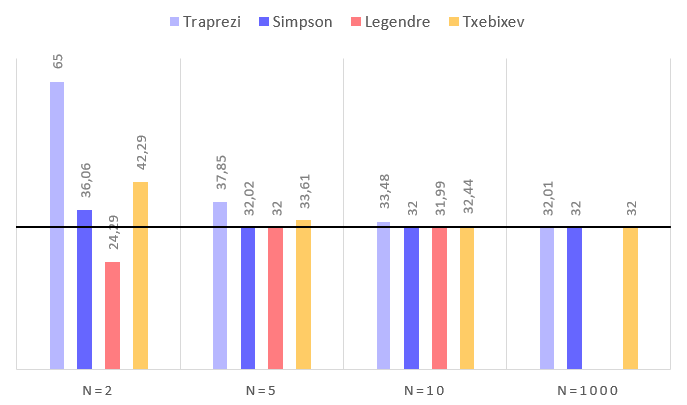
\includegraphics[width = 0.75\textwidth]{excelsupremacy.png}
    \caption{Resultats depenent del nombre de subintervals}
    \label{fig:my_label}
\end{figure}\\
La linia negra senyala el valor real de l'integral; és a dir $32$.\\
Els resultats obtinguts per al valor de $n\in\{2,5,10,1000\}$ demostren que, efectivament, la precisió dels mètodes augmenta a mida que augmenta el valor del nombre d'intervals.\\
Fer èmfasi que per a un valor de $n\not\in\{2,5,10\}$ el mètode de Legendre no funciona, per falta d'informació en memòria sobre els pesos i els valors de les $x$ a escollir, pel que amb $n=1000$ no apareix el seu resultat.\\
Resaltar, a més, que sembla ser que el mètode que millor s'adapta per a calcular els valors de les integrals per a cualsevol valor de $n$ és el mètode de Simpson Compost; ja que veiem com s'apropa ràpidament al valor real per a un valor de $n$ relativament petit (com ho és el valor de $n=5$).


\newpage
\section{Compilació i execució}
\subsection{Compilació del Programa}
\subsubsection{Makefile}
Per facilitar la compilació del programa s'ha creat un fitxer $makefile$ que inclou tant les comandes per crear l'executable com altres comandes associades ($clean$ i $clean\_all$ que explicarem més endavant) per la correcta gestió dels fitxers que s'obtenen de l'execució del makefile.\\
Per compilar el programa i generar l'executable ($gauss$) només cal escriure a la terminal on es troben tots els fitxers (inclós el $makefile$) la comanda make: 
\begin{verbatim}
    $make
\end{verbatim}
Com hem comentat anteriorment, el fitxer makefile també conté comandes per la correcta gestió dels fitxers resultants d'obtenir l'executable, aquestes comandes són:
\begin{verbatim}
    $make clean
    $make clean_all
\end{verbatim}
La comanda $clean$ elimina tots el fitxers $.o$ del directori mentre que la comanda $clean\_all$ elimina tant l'executable com els fitxers amb terminació $.o$.\\
Mencionar que no es poden utilitzar les dues comandes de manera seguida ja que donarà error.\\
\textbf{Important:} en cas de no utilitzar el sistema operatiu $Linux$ (o semblants) o $IOS$ cal modificar la variable $DELETE$ de l'arxiu $makefile$ per a poder utilitzar-lo (substituir per la comanda $del$ en cas d'utilitzar Windows).

\subsubsection{Compilació manual}
En cas de voler compilar el programa de manera manual (comanda a comanda) utilitzar en ordre les comandes al terminal (una vegada ubicat al directori on es troben els fitxers).
\begin{verbatim}
    $gcc -c integracio.c integracio.h -lm
    $gcc -c gauss.c  integracio.c -lm 
    $gcc gauss.o  integracio.o -lm -o gauss
\end{verbatim}

\subsection{Execució del programa}\label{execucio}
Un cop s'ha compilat el programa, per executar-lo cal escriure a la terminal la comanda \texttt{\$./gauss} $ \mu$ $\sigma^2$ \texttt{x}; on els valors $\mu$, $\sigma^2$ son els els paràmetres d'una distribució aleatòria Normal $(\hspace{0.5em}X \sim N(\mu,\sigma^2)\hspace{0.5em})$.\\
Per altra banda, la x és el valor pel qual es calcularà $P(|X|>x)$.\\
\begin{figure}[h]
    \centering
    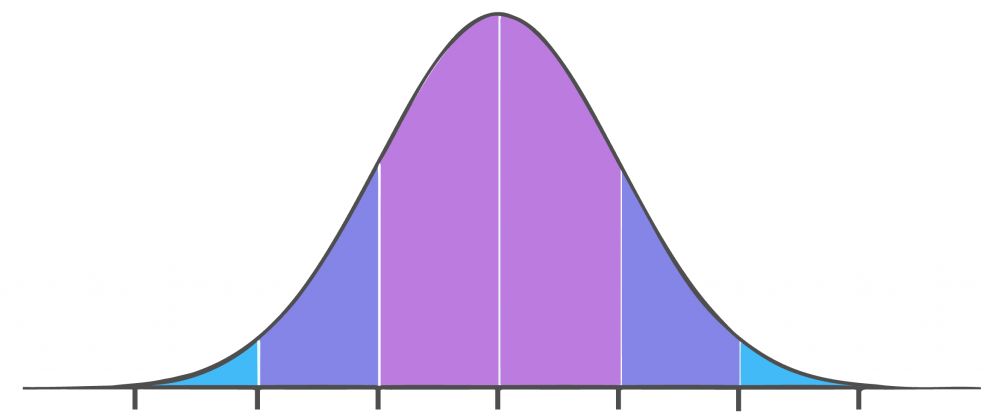
\includegraphics[width = 0.75 \textwidth]{normalcuquibuena.PNG}
    \caption{Representació de l'àrea de les cues de la distribució normal}
    \label{fig:my_label}
\end{figure}\\
Si s'executa el programa amb aquesta comanda, el valor per defecte de n (nombre de subintervals que s'utilitza per calcular la integral) és 10. \\
El programa està pensat per poder executar-se també amb la comanda: \texttt{\$./gauss} $ \mu$ $\sigma^2$ \texttt{x n}, on n és el nombre de subintervals, per si es vol calcular amb un valor diferent a 10.\\
Si s'introdueixen menys dels 3 paràmetres imprescindibles ($\mu$, $\sigma^2$ i \texttt{x}) es mostrarà un missatge d'error, mentre que si s'introdueixen més de 4 valors ($\mu$, $\sigma^2$, \texttt{x} i \texttt{n}), el programa ignorarà els que hi hagi de més.\\
Una vegada executat el programa es mostrarà per \texttt{stdout} el valor de la probabilitat (calculada pels quatre mètodes que inclou la llibreria).\\\\
\textit{Cal fer especial menció en que el programa gauss.c només gestiona que els valors introduïts per l'equació de la distribució gaussiana tinguin sentit (que s'hagin introduït $\mu\in\mathbb{R}$, $x, \sigma^2\in\mathbb{R^+}$); que el valor del nombre de subintervals introduït sigui correcte és gestionat per la llibreria}.
\newpage

\section{Explicació Gauss}
Recordem que el programa Gauss (mitjançant la llibreria \textcolor{LimeGreen}{integracio.h} ja esmentada) calcula l'àrea dels extrems d'una distribució normal amb paràmetres $\mu, \sigma^2$ (és a dir; si $X \sim N(\mu,\sigma^2)$, retorna $P(|X|> x)$; per a $x\in \mathbb{R^+}$ el valor desitjat).\\
Per a l'execució i introducció de les dades es recomana llegir l'apartat anterior (secció \textcolor{blue}{\ref{execucio}}).\\
 A continuació és mostraran diversos resultats obtinguts per a la comprovació del correcte funcionament del programa i la seva deguda anàlisi.
\subsection{Exemplificació del programa \texttt{gauss.c}}\label{gauss}
Suposarem en aquest apartat 3 casos pels que serveix i és útil la nostra llibreria.
\begin{itemize}
    \item\textbf{Experiment amb resultat} $x=\mu+5\sigma$:\\
    Suposem que en un donat experiment obtenim que els resultats pertanyen a l'interval $[-x,x]$ on $x=\mu+5\sigma$, essent $\mu,\sigma^2$ els paràmetres d'una distribució normal (més concretament, $\mu=-5, \sigma^2 = 16$; és a dir, $N(-5,16)$).\\
    Volem saber si la mostra obtinguda està continguda en un interval amb alta probabilitat o, si per el contrari no ho està (fet que podria suposar algun problema experimental o de plantejament de l'experiment).\\
    Per tant, volem saber $P(|N(-5,16)|> -5 + 5\cdot 4 = 15)$.
    Els valors obtinguts són:
    \begin{verbatim}
        Area Trapezi --> 0.006437551475070247
        Area Simpson --> 0.006210149190216119
        Area Legendre--> 0.006209368495169398
        Area Txebixev--> 0.001042226044340622
    \end{verbatim}
    Observem doncs que la probabilitat d'haver obtingut valors fora de l'interval és suficientment petita com per afirmar que segueix una distribució normal.
    \newpage
    \item \textbf{Càlcul del p-value}:\\
    Suposem que tenim dues poblacions independents que segueixen una distribució normal de la qual sabem els valors de $\sigma_x^2$ i $\sigma_y^2$ i volem fer un test d'hipòtesis per saber si $\mu_x = \mu_y$, amb un nivell de significació $\alpha$ = 0.05.\\
     Rebutjarem la hipòtesis inicial ($\mu_x = \mu_y$) si el p-valor és menor a $\alpha$.\\
    Per fer el test d'hipòtesis, lo primer que hauríem de fer és calcular el test estadístic $W(x) \sim N(0,1)$.\\ 
    Suposem $W(x) = 2.3$.\\
    El càlcul del p-valor és la probabilitat d'obtenir un valor més extrem o igual a l'observat $W(x)$, és a dir, $P(|N(0,1)|> 2.3)$.\\
    Els valors del p-valor obtinguts són:
    \begin{verbatim}
        Area Trapezi --> 0.022021479049143755
        Area Simpson --> 0.021448511966331518
        Area Legendre--> 0.021440498451698042
        Area Txebixev--> 0.018104816983536998
    \end{verbatim}
    Per tant, rebutgem la hipòtesis inicial.
    \begin{figure}[h]
        \centering
        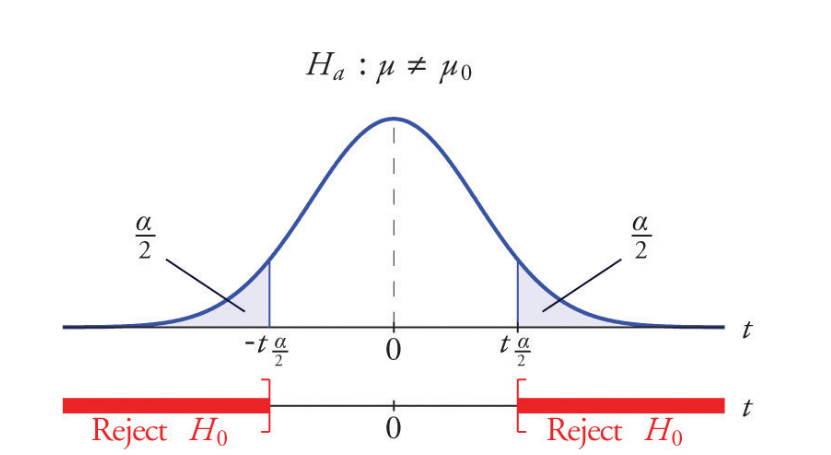
\includegraphics[width = 0.8\textwidth]{rechazarbrrr.PNG}
        \caption{Regió de rebuig d'una distribució normal per a un valor $t$.}
        \label{fig:my_label}
    \end{figure}
    \newpage
    \item \textbf{Detecció de valors \textit{outliers}}:\\
    Suposem que volem modelitzar un sistema que creiem que segueix una distribució normal amb paràmetres $(\mu,\sigma^2) = (0,1)$.\\
    Ens percatem que de les mostres que hem obtingut totes excepte $1$ es troben dins l'interval $[-2,2]$, l'excepció es situa a $x=-2.5$. \\
    Volem saber quina és la probabilitat de que el fenòmen que provoca aquest resultat sigui suficientent gran com per a tenir-lo en compte; o si pel contrari podem descartar-lo per simplificar la nostra representació.\\
    Sabem, per tant, que un fenòmen més extrem a aquest està contingut a l'interval $(-\infty,-2.5]\cup[2.5,+\infty)$; pel que calculem la probabilitat (segons el nostre model) que succeeixi un d'aquests fenòmens extrems, és a dir, $P(|N(0,1)|>2.5)$.\\
    Els valors obtinguts són:
    \begin{verbatim}
        Area Trapezi --> 0.012874245540560880
        Area Simpson --> 0.012419718839867366
        Area Legendre--> 0.012413827204901917
        Area Txebixev--> 0.008876008616628128
    \end{verbatim}
    Ens percatem que la probabilitat d' enregistrar en l'experiment un fenòmen similiar o més extrem al obtingut és suficientment petita (una mica superior al $1\%$) com per a tractar aquest resultat com \textit{outlier}. Per tant podem no utilitzar-lo per a fer el nostre model més senzill.\\
    \begin{figure}[h]
        \centering
        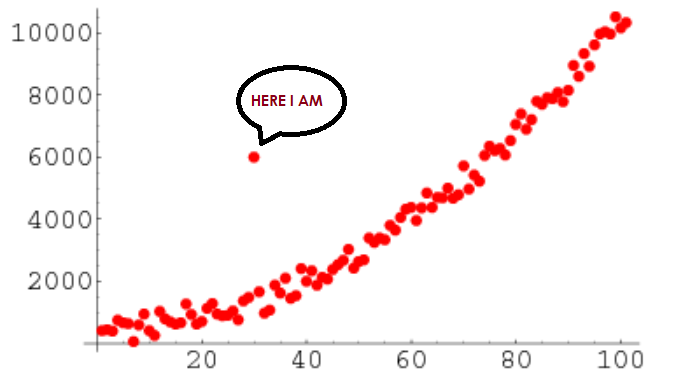
\includegraphics[width = 0.49\textwidth]{outlier.png}
        \caption{Exemplificació d'un outlier qualsevol.}
        \label{fig:my_label}
    \end{figure}
    
\end{itemize}

\newpage
\section{Conclusions}
Finalitzem l'informe afirmant (a partir de les dades experimentals dutes als apartats \textcolor{blue}{\ref{comprovacions}} i \textcolor{blue}{\ref{gauss}} que tant la biblioteca \textcolor{LimeGreen}{integració.c} com el programa \texttt{gauss.c} funcionen de manera correcta llevat de petits errors deguts a la precisió de la màquina.\\
Tot i així les aproximacions de les integrals són suficientment bones com per recomanar l'ús de la llibreria.\\
Recomanem de la mateixa manera que es calculin les integrals mitjançant els quatre mètodes d'integració per a obtenir una millor aproximació i/o un cert interval de confiança.
\subsection{Informació adicional}
\begin{itemize}
    \item Informar que en cas d'obtenir una àrea menor d'una certa tolerància el programa interpretarà aquella àrea com a 0 (la tolèrancia introduïda és de $10^{-10}$ que és on hem observat experimentalment que existeix més perill d'error d'aproximació amb tendències a desplaçar el valor al semieix negatiu).

    \item La complexitat dels mètodes són d'ordre lineal; és a dir, $O(n)$ (on $n$ és el nombre de subintervals).

    \item Responem a la pregunta: \textbf{Com generarieu una variable
aletòria normal utilitzant les llibreries bàsiques de C?}\\
C permet generar variables aleatòries, però segueixen únicament una distribució uniforma. Per poder generar una distribució normal, s'haurà de fer ús de la comanda \texttt{rand}.\\
Per simular una distribució normal amb mitja $\mu$ i variança $\sigma^2$ es necessita utilitzar la interpretació del teorema del límit central: 
\begin{equation*}
    \lim_{N \to \infty} P\left(\frac{\sum_{i=1}^{n} U_{i} - N\mu }{\sqrt{N}\sigma} \in (a,b) \right) = \frac{1}{\sqrt{2\pi}} \bigintsss_{a}^{b} e^{\frac{-x^2}{2}} dx
\end{equation*}
On $U_i\sim Uniforme(\mu)$ (segueix una distribució uniforme d'esperança $\mu$, centrada a $\mu$, que centrarà la distribució normal a aquest valor) i $\sigma^2$ és la desviació que volem que tingui la distribució normal.\\
Per obtenir una distribució normalitzada (de mitja 0 i desviació típica 1) cal seguir els següents passos:
\begin{enumerate}
    \item Generar $n$ mostres uniformes, amb valors continguts a l'interval $[-0.5,0.5]$ (és a dir, $P(x\in[-0.5,0.5])=1$ i $P(x\not\in[-0.5,0.5])=0$), i una esperança nul·la (centrada a l'origen).
    \item Crear una nova variable aleatòria, sumant totes les mostres. Aquesta nova variable aleatòria segueix una distribució normal per valors de $n$ grans.
    \item Realitzar aquests passos un nombre gran de cops, de manera que poguem verificar que segueix una distribució normal. 
\end{enumerate}
\end{itemize}


































\end{document}
